\title{7. Goniometrické funkce}
\author{Jakub Švagr}
\date{1.5.2025}

\maketitle

\section{Goniometrické funkce}
Jsou skupinou funkcí, které dávají do vztahu úhel v pravoúhlém trojúhelníku a poměr dvou jeho stran. \\\\ 
\subsection{Jednotková kružnice}
Jednotková kružnice je kružnice se středem v počátku souřadnic a o poloměru 1\\\\ 
Hodnoty goniometrických funkcí nalezneme v tabulkách. Jsou tradičně udávány ve stupních $^\circ$, nebo radiánech $\pi$.
\begin{figure}[H]
        \centering
        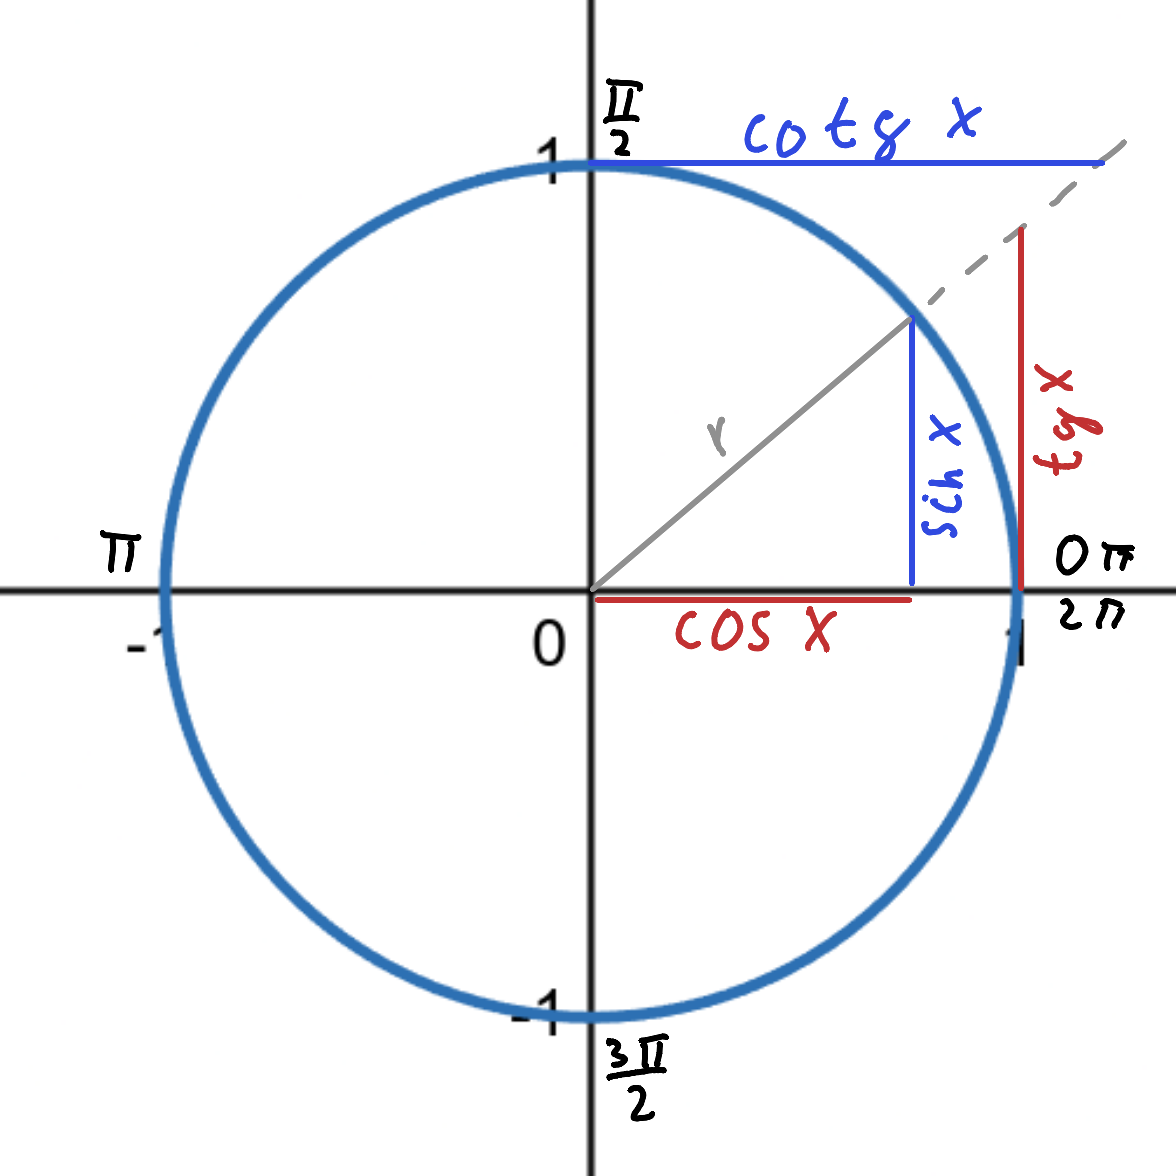
\includegraphics[width=0.6\linewidth]{img/7_JednotkovaKruznice.png}
        \caption{Jednotková Kružnice} 
        \label{fig:Jednotková Kružnice}
\end{figure}
Funkce jsou periodické, což znamená, že se jejich hodnoty pravidelně opakují (jako na kruhu)
\subsection{Grafy funkcí}
\subsubsection{Sinus a Kosinus}
\begin{figure}[H]
        \centering
        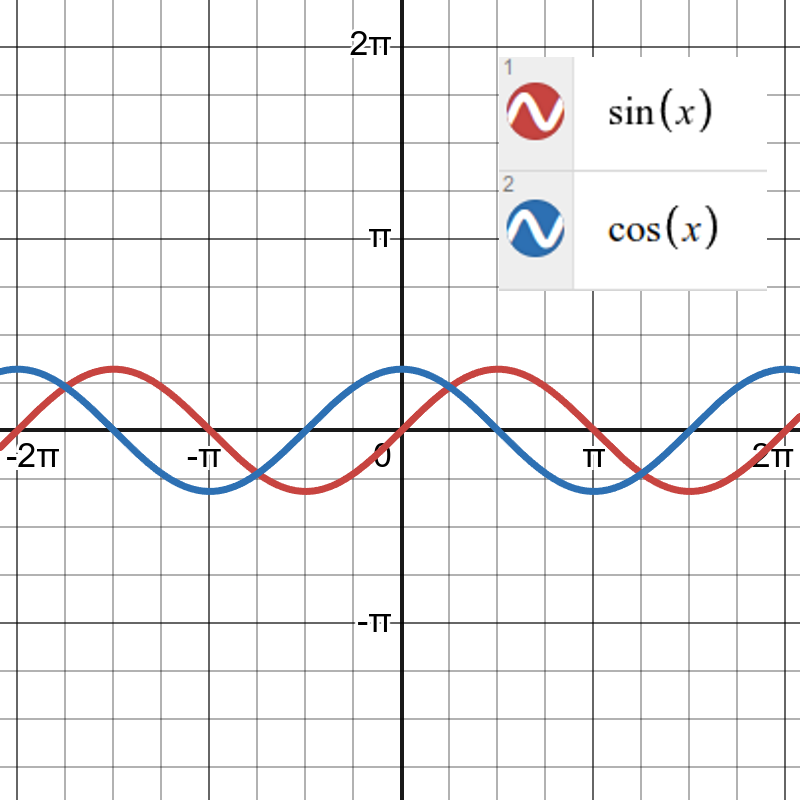
\includegraphics[width=0.5\linewidth]{img/7_SinXCosX.png}
        \caption{$f(x): y=sin(x), g(x): y=cos(x)$} 
        \label{fig:Graf rovnice sin(x) a cos(x)}
\end{figure}

sin(x) začíná v počátku, tedy v bodě [0;0] (na grafu znázorněn červeně). Je to lichá funkce (souměrná podle počátku, jako jediná goniometrická funkce)  periodická v intervalu $\langle0; 2\pi\rangle$. Je definována v pravoúhlém trojúhelníku, jako poměr délky protilehlé odvěsny úhlu alfa ku délce přepony:
$$
    \sin\alpha=\frac{\text{délka protilehlé odvěsny úhlu alfa}}{\text{délka přepony}}
$$
\begin{figure}[h]
    \centering
    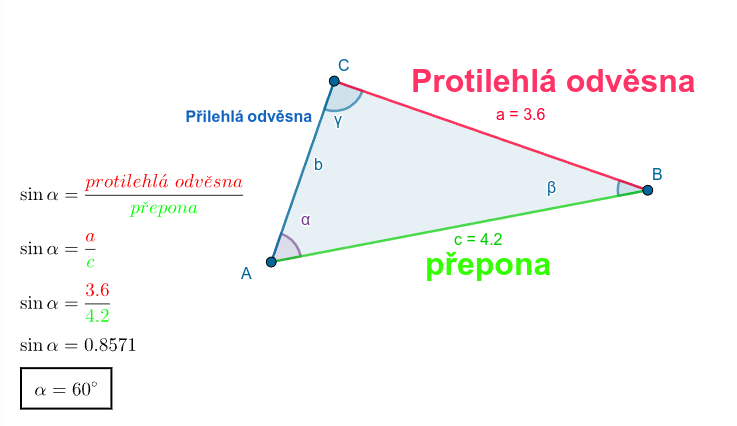
\includegraphics[width=0.5\linewidth]{img/7_TrojuhlenikASinus.png}
    \caption{$\sin \alpha$, znázorněn na pravoúhlém trojúhelníku}
    \label{fig:sinus-na-pravouhlem-trojuhelniku}
\end{figure}
cos(x) začíná v bodě [0;1] (na grafu znázorněn modře), je  to sudá funkce (souměrná podle osy x) a periodická v intervalu $\langle0; 2\pi\rangle$. Je definována v pravoúhlém trojúhelníku, jako poměr délky přilehlé odvěsny úhlu alfa ku délce přepony:
$$
    \cos\alpha=\frac{\text{délka přilehlé odvěsny úhlu alfa}}{\text{délka přepony}}
$$
\begin{figure}[h]
    \centering
    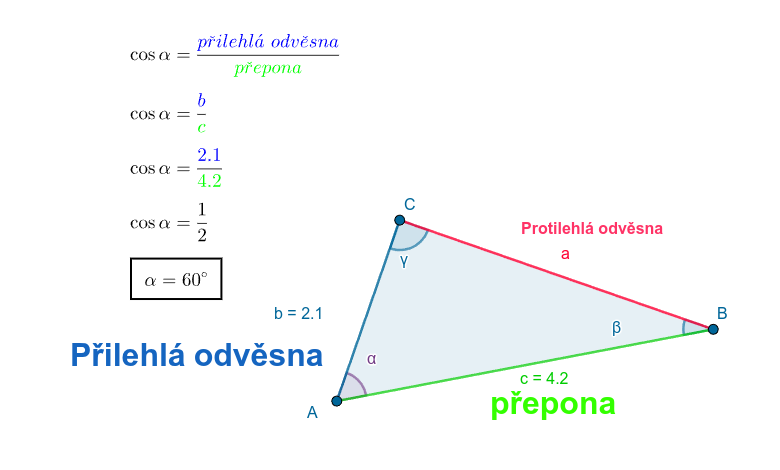
\includegraphics[width=0.5\linewidth]{img/7_TrojuhlenikAKosinus.png}
    \caption{$\cos \alpha$, znázorněn na pravoúhlém trojúhelníku}
    \label{fig:kosinus-na-pravouhlem-trojuhelniku}
\end{figure}
\subsubsection{Tangens a Kotangens}
\begin{figure}[H]
        \centering
        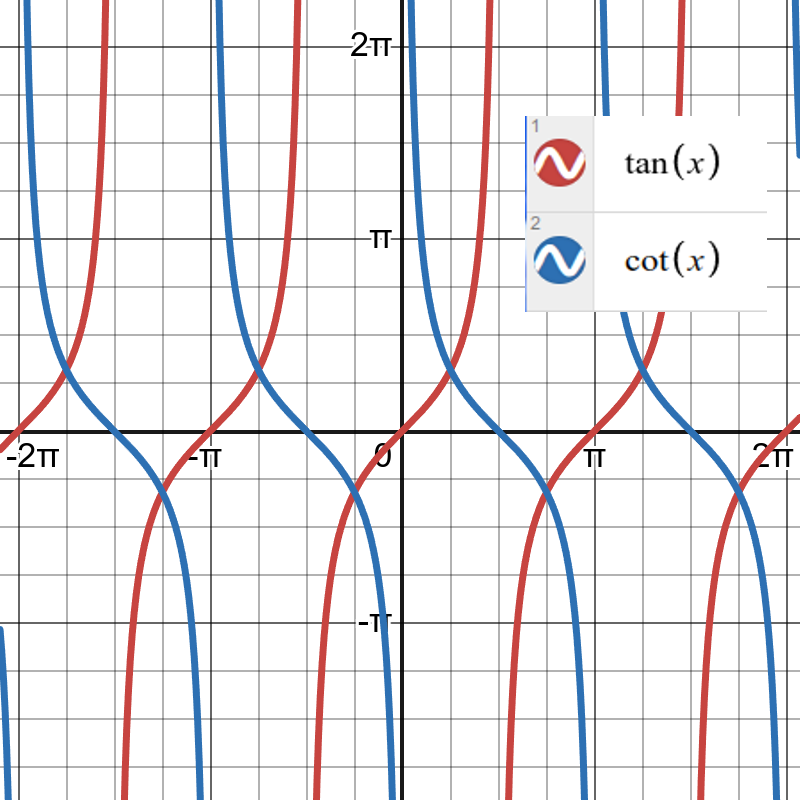
\includegraphics[width=0.5\linewidth]{img/7_TgXCotgX.png}
        \caption{$f(x): y=tg(x), g(x): y=cotg(x)$} 
        \label{fig:Graf rovnice tg(x) a cotg(x)}
\end{figure}

tg(x), na grafu červeně, je funkce periodická v intervalu $\pi$ (o polovinu méně než sin(x) a cos(x)), lichá, definovaná v intervalu $(-\frac{\pi}{2};\frac{\pi}{2})$ je definována jako poměr:
$$
    tg(x) = \frac{\sin(x)}{\cos(x)}
$$
V pravoúhlém trojúhelníku odpovídá poměru délky protilehlé odvěsny ku přilehlé odvěsně:
$$
    tg(x) = \frac{\text{protilehlá odvěsna}}{\text{přilehlá odvěsna}}
$$
Tangens není definován pro ty úhly, kdy je $\cos(x) = 0$, takže \textbf{neexistuje} $tg\left(\frac{\pi}{2} + k\pi\right)$, neboli $90^{\circ}+ k \times 180^{\circ}$ kde $k \in \mathbb{Z}$. 

\begin{figure}[h]
    \centering
    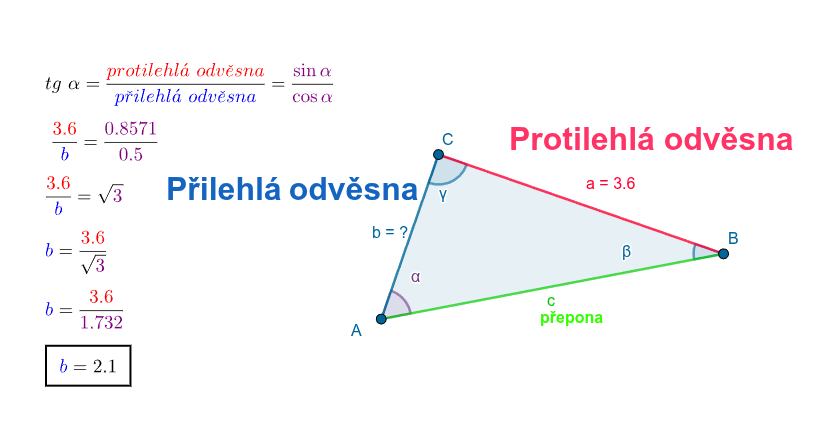
\includegraphics[width=0.5\linewidth]{img/7_TrojuhlenikATangens.png}
    \caption{$tg\ \alpha$, znázorněn na pravoúhlém trojúhelníku}
    \label{fig:tangens-na-pravouhlem-trojuhelniku}
\end{figure}

cotg(x), na grafu modře, je taktéž periodická funkce s periodou $\pi$, a je definována jako poměr:
$$
    cotg(x) = \frac{\cos(x)}{\sin(x)}
$$
V pravoúhlém trojúhelníku představuje poměr délky přilehlé odvěsny ku protilehlé odvěsně:
$$
    cotg(x) = \frac{\text{přilehlá odvěsna}}{\text{protilehlá odvěsna}}
$$
Kotangens není definován pro ty úhly, kdy je $\sin(x) = 0$, takže \textbf{neexistuje} $cotg(k\pi)$, neboli $0^{\circ}+ k \times 180^{\circ}$ kde $k \in \mathbb{Z}$
\begin{figure}[h]
    \centering
    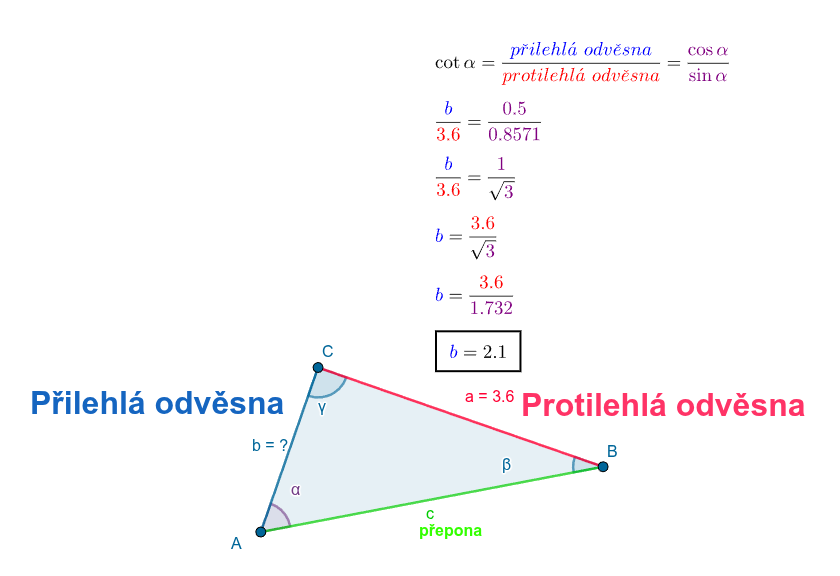
\includegraphics[width=0.5\linewidth]{img/7_TrojuhlenikAKotangens.png}
    \caption{$cotg\ \alpha$, znázorněn na pravoúhlém trojúhelníku}
    \label{fig:kotangens-na-pravouhlem-trojuhelniku}
\end{figure}
\subsection{Tabulky}
\begin{table}[h]
    \centering
    \begin{tabular}{|c|c|c|c|c|c|}
        \hline
        \multicolumn{2}{|c|}{\textbf{ÚHLY}} & \multicolumn{4}{c|}{\textbf{GON. FUNKCE}} \\ \hline
        $\alpha^\circ$ & $\alpha$ (rad) & $\sin \alpha$ & $\cos \alpha$ & $\tan \alpha$ & $\cot \alpha$ \\ \hline
        $30^\circ$ & $\frac{\pi}{6}$ & $\frac{1}{2}$ & $\frac{\sqrt{3}}{2}$ & $\frac{\sqrt{3}}{3}$ & $\sqrt{3}$ \\ \hline
        $45^\circ$ & $\frac{\pi}{4}$ & $\frac{\sqrt{2}}{2}$ & $\frac{\sqrt{2}}{2}$ & 1 & 1 \\ \hline
        $60^\circ$ & $\frac{\pi}{3}$ & $\frac{\sqrt{3}}{2}$ & $\frac{1}{2}$ & $\sqrt{3}$ & $\frac{\sqrt{3}}{3}$ \\ \hline
    \end{tabular}
    \caption{Hodnoty  goniometrických funkcí}
    \label{tab:Goniometricke_Funkce}
\end{table}

\begin{table}[h]
    \centering
    \begin{tabular}{|c|c|c|c|c|}
    \hline
    \textbf{Kvadrant} & sin(x) & cos(x) & tg(x) & cotg(x) \\ \hline
    I.  & + & + & + & + \\ \hline
    II. & + & -- & -- & -- \\ \hline
    III.& -- & -- & + & + \\ \hline
    IV. & -- & + & -- & -- \\ \hline
    \end{tabular}
    \caption{Tabulka znamének pro kvadranty}
    \label{tab:Znamenka_Goniometrie}
\end{table}
\subsection{Jak na to?}
\subsubsection{Sinus a Kosinus}
Je dobré pro orientaci použít jednotkovou kružnici, jde to udělat i bez ní, ale pokud se opravdu chcete vyhnout chybě, tak se hodí. Jako jednoduchý příklad jsem použil hodnotu $\sin(x) = \frac{1}{2}$.
\begin{enumerate}
    \item Hledáme všechny hodnoty $x$, pro které platí $\sin(x) = \frac{1}{2}$.
    
    \item Teď se podíváme do tabulky, z toho zjistíme že pro $\frac{1}{2}$ je $\sin{\frac{\pi}{6}}$:
    \[
    \sin\left(\frac{\pi}{6}\right) = \frac{1}{2}
    \]
    To znamená, že jeden z úhlů, který tuto rovnici splňuje, je $\frac{\pi}{6}$.

    \item ALE funkce sinus je kladná i ve druhém kvadrantu, existuje ještě druhý úhel s touto hodnotou, jak je vidět na jednotkové kružnici:
    \begin{figure}[H]
        \centering
        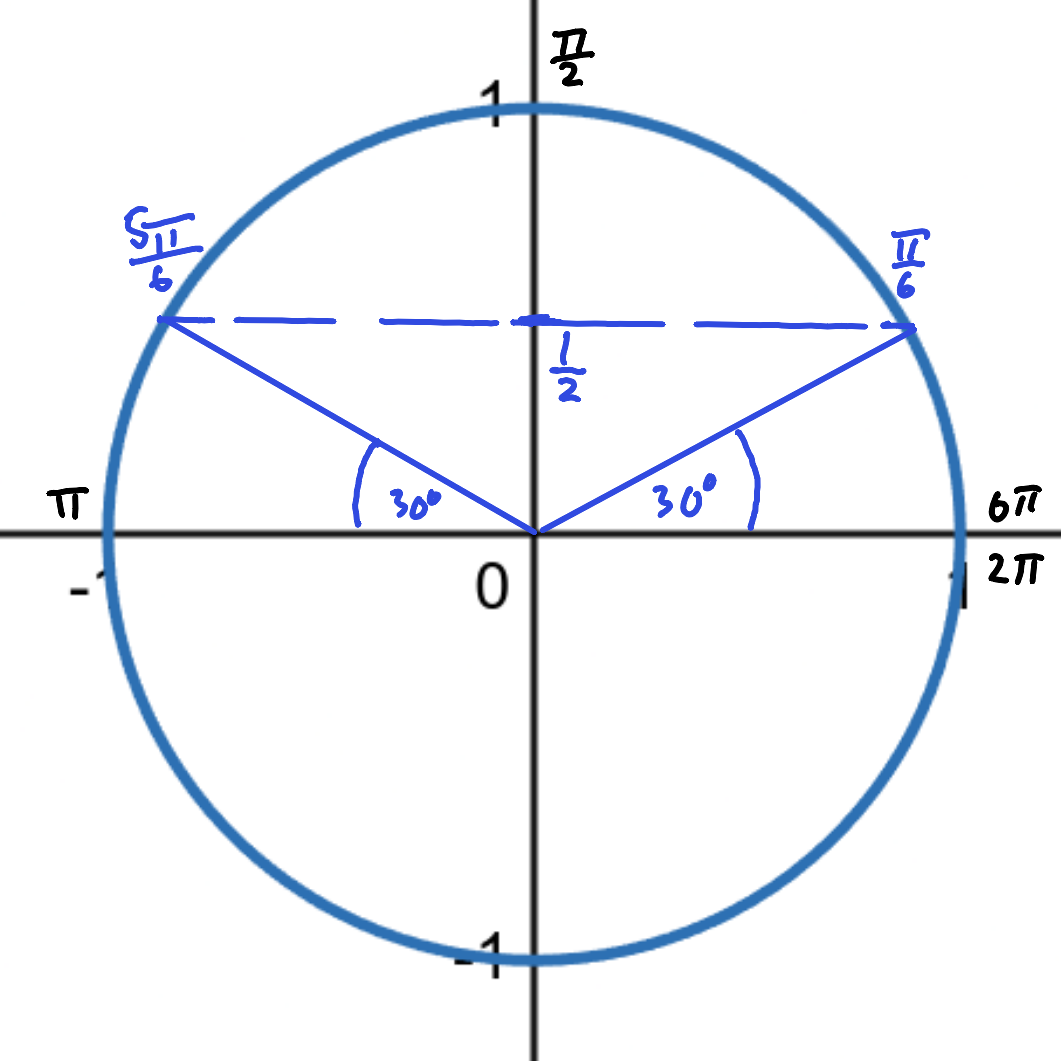
\includegraphics[width=0.4\linewidth]{img/7_JednotkovaKruzniceSinpolovina.png}
        \caption{$\sin{\frac{1}{2}}$} 
        \label{fig:Sinus jedné poloviny na jednotkové kružnici}
\end{figure}
    \[
    x = \pi - \frac{\pi}{6} = \frac{5\pi}{6}
    \]

    \item Funkce sinus je periodická s periodou $2\pi$, takže obecné řešení je:
    \[
    x_1 = \frac{\pi}{6} + 2k\pi \quad, \quad x_2 = \frac{5\pi}{6} + 2k\pi, \quad k \in \mathbb{Z}
    \]
\end{enumerate}
V případě že počítáme funkci $cos(x)$, postup je stejný, jediný rozdíl je, že místo osy $y$ použijeme osu $x$, a to takto:
\begin{figure}[H]
        \centering
        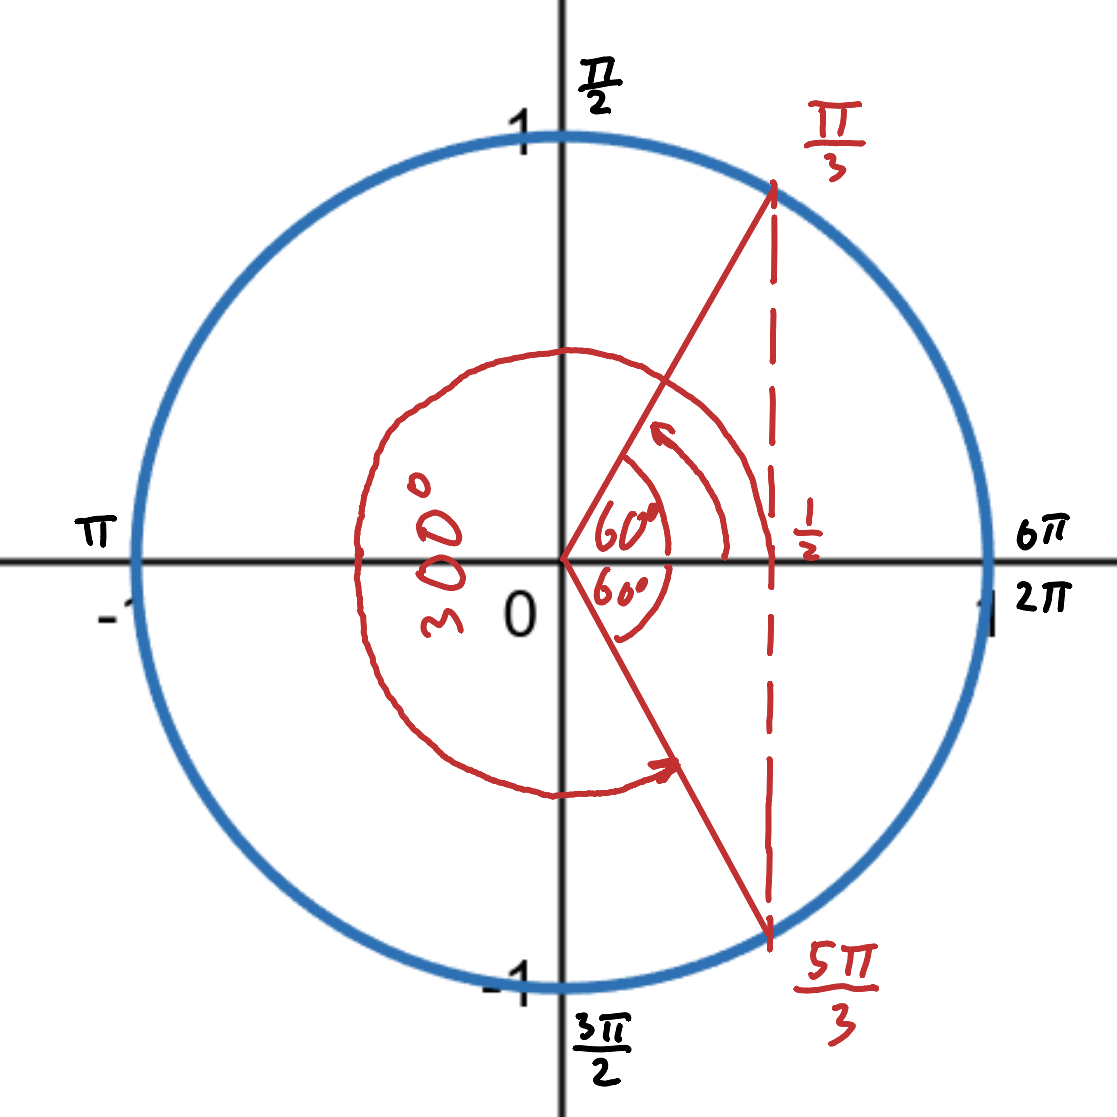
\includegraphics[width=0.4\linewidth]{img/7_JednotkovaKruznicekosinuspolovina.png}
        \caption{$\cos{\frac{1}{2}}$} 
        \label{fig:Kosinus jedné poloviny na jednotkové kružnici}
\end{figure}
\subsubsection{Tangens a Kotangens}
Tito dva se zdají být výrazně děsivější, ale jakmile to pochopíte, je to vcelku jednoduché, tady je příklad s tabulkovou hodnotou:
\begin{enumerate}
    \item Hledáme hodnoty $x$, pro které platí $\tan(x) = \sqrt{3}$.

    \item Když se podíváme to tabulky, zjistíme že:
    \[
    \tan\left(\frac{\pi}{3}\right) = \sqrt{3}
    \]
    Takže jeden z úhlů, který tuto rovnici splňuje, je:
    \[
    x = \frac{\pi}{3}
    \]
    \begin{figure}[H]
        \centering
        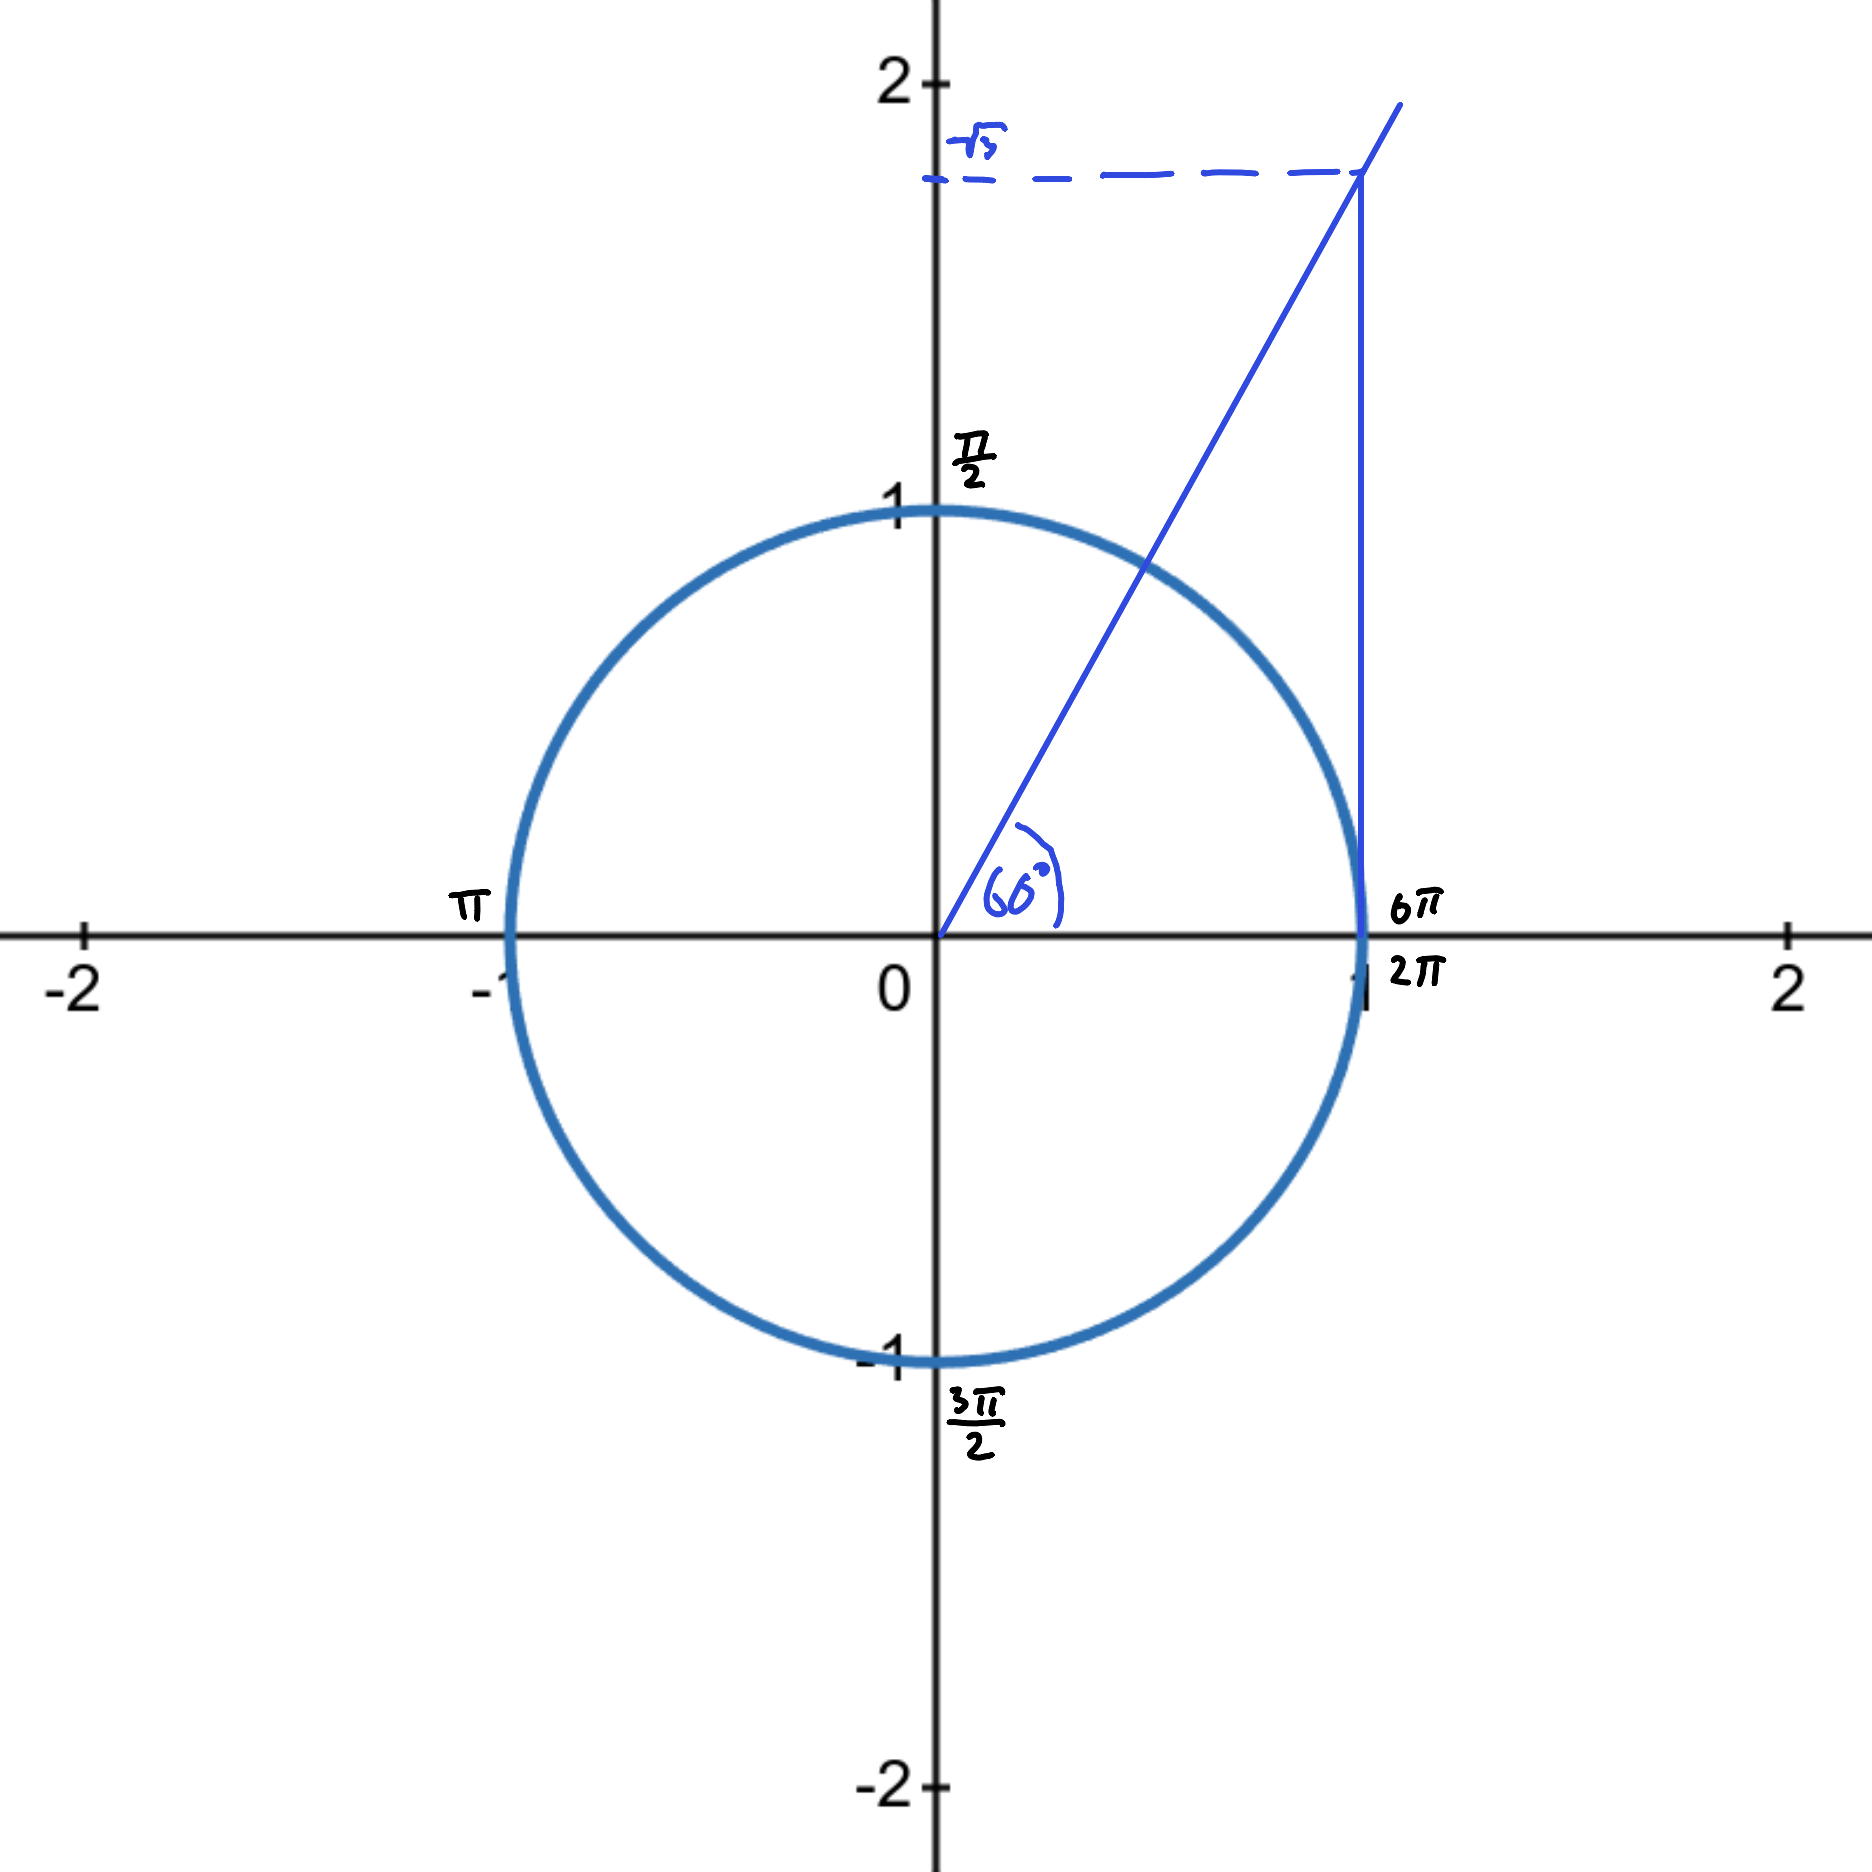
\includegraphics[width=0.5\linewidth]{img/7_JednotkovaKruzniceTangens.png}
        \caption{$tg\sqrt{3}$} 
        \label{fig:Tangens jedné poloviny na jednotkové kružnici}
\end{figure}

    \item Funkce tangens má periodu $\pi$, protože se opakuje každých 180° (ne každých $2\pi$ jako sinus a kosinus), také je na rozdíl od nich kladný v protilehlých kvadratech, tedy v prvním a třetím kvadrantu. O to je naše práce jednoduší, jak jsem znázornil na jednotkové kružnici, stačí pouze z naši polopřímku protáhnout na druhou stranu.
%Tento obrázek může klidně být místo toho prvního, poté by se to všechno vlezlo na stránku, je na tobě jestli si myslíš, že to tady je dobré nechat.
    \begin{figure}[H]
        \centering
        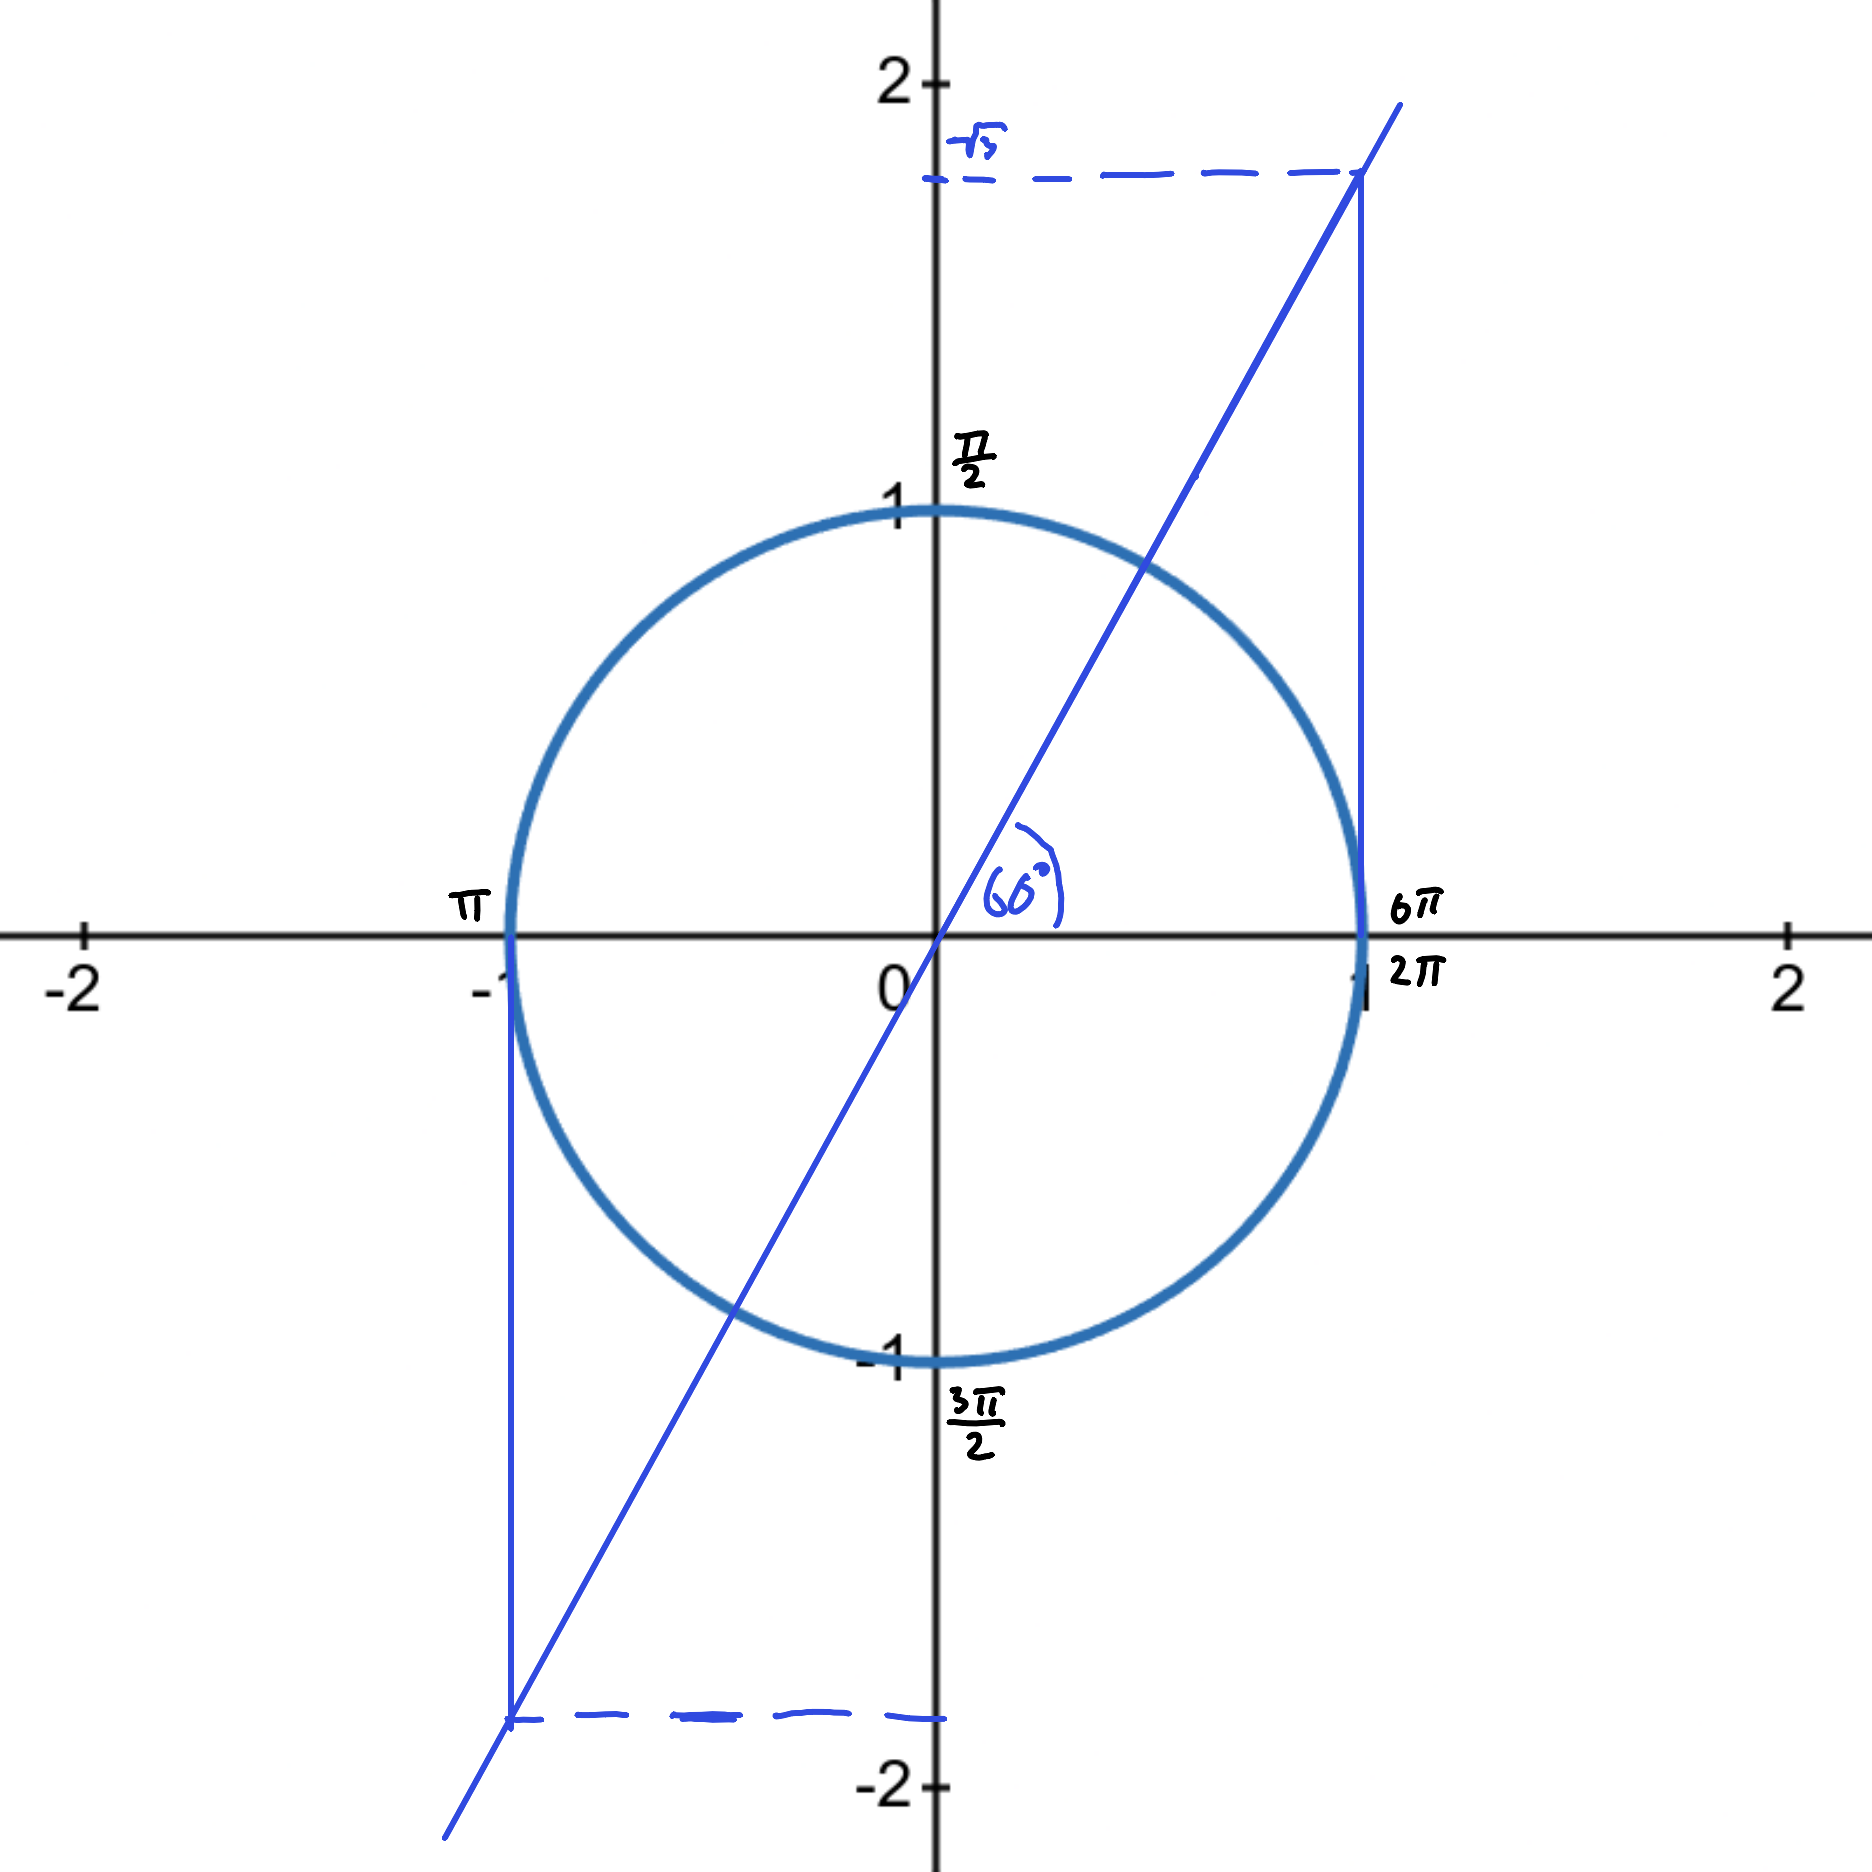
\includegraphics[width=0.5\linewidth]{img/7_JednotkovaKruzniceTangensKomplet.png}
        \caption{$tg\sqrt{3}$} 
        \label{fig:Tangens jedné poloviny na jednotkové kružnici, dokončeno}
    \end{figure}
    \item Taky je dobré si všimnout, že $\sqrt{3} > 1$, toto je možné pouze proto, že $tg(x)$ a $cotg(x)$ mohou dosahovat $-\infty$ až $+\infty$, vyjma tedy těch hodnot, kdy by hodnota ve jmenovateli byla rovna $0$.

    \item Obecné řešení rovnice tedy je:
    \[
    x = \frac{\pi}{3} + k\pi, \quad k \in \mathbb{Z}
    \]

\end{enumerate}
V případě funkce $cotg(x)$ je to podobné jako u kosinu.